% ------------------------------------------------------------------------------
% TYPO3 Version 9.1 - What's New - Chapter "Changes for Integrators" (English Version)
%
% @author	Michael Schams <schams.net>
% @license	Creative Commons BY-NC-SA 3.0
% @link		http://typo3.org/download/release-notes/whats-new/
% @language	English
% ------------------------------------------------------------------------------
% LTXE-CHAPTER-UID:		3a9852ea-e2360d9d-1ff5eec1-a7de3f9f
% LTXE-CHAPTER-NAME:	Changes for Integrators
% ------------------------------------------------------------------------------

\section{Änderungen für Integratoren}
\begin{frame}[fragile]
	\frametitle{Änderungen für Integratoren}

	\begin{center}\huge{Kapitel 2:}\end{center}
	\begin{center}\huge{\color{typo3darkgrey}\textbf{Änderungen für Integratoren}}\end{center}

\end{frame}

% ------------------------------------------------------------------------------
% LTXE-SLIDE-START
% LTXE-SLIDE-UID:		31b70474-edcc2a8a-d4a5fd3d-58734dc5
% LTXE-SLIDE-TITLE:		EXT:impexp - Maximum Number Of Records Restriction Removed
% LTXE-SLIDE-REFERENCE:	Deprecation-83592-ImpexpRemovedMaximumNumberOfRecordsRestriction
% ------------------------------------------------------------------------------

\begin{frame}[fragile]
	\frametitle{Änderungen für Integratoren}
	\framesubtitle{Import/Export}

	Diverse Updates an der Systemerweiterung \texttt{impexp}:

	\begin{itemize}
		\item Die Beschränkung "maximale Anzahl von Datensätzen" wurde entfernt\newline
			\smaller
				Die Obergrenze beim Exportieren von Seiten oder Datensätzen wurde entfernt.
			\normalsize

		\item Die Beschränkung "maximale Dateigröße" wurde entfernt\newline
			\smaller
				Die Limitierung der Dateigrößen über die
				"Exportieren"-Oberfläche wurde entfernt.
			\normalsize

		\item Größenbehandlung wurde entfernt\newline
			\smaller
				Beim Exportieren oder Importieren von Datenstrukturen wurden Größeninformationen für     
				Datensätze und Dateien in der Exportdatei erfasst und beim Import validiert.
				Diese Änderung hat keine Auswirkung auf Redakteure.
			\normalsize
	\end{itemize}

\end{frame}

% ------------------------------------------------------------------------------
% LTXE-SLIDE-START
% LTXE-SLIDE-UID:		0504ca33-7c23eff4-93a728fa-bd911c92
% LTXE-SLIDE-TITLE:		Redirect Functionality Moved To Redirects Module
% LTXE-SLIDE-REFERENCE:	83638-RedirectFunctionalityMovedFromSys_domainToRedirectsModule
% ------------------------------------------------------------------------------

\begin{frame}[fragile]
	\frametitle{Änderungen für Integratoren}
	\framesubtitle{Weiterleitungsfunktionalität}

	\begin{itemize}
		\item Die Option eine Weiterleitung innerhalb eines Domain Records einzurichten wurde entfernt.
		\item Das Einrichten von Weiterleitungen kann jetzt im neuen Modul \newline
			\textbf{Site Management} \textrightarrow \textbf{Redirects} erstellt werden
	\end{itemize}

	\begin{figure}
		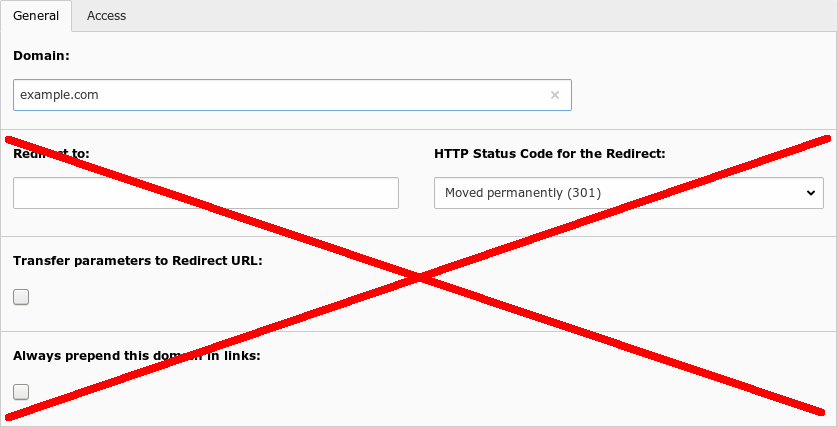
\includegraphics[width=0.6\linewidth]{ChangesForIntegrators/RedirectFunctionalityMovedToRedirectsModule.png}
	\end{figure}

\end{frame}

% ------------------------------------------------------------------------------
